\documentclass[../poma-notes.tex]{subfiles}

\begin{document}

\subsection*{Discontinuities}

如果 $x$ 是位于函数 $f$ 所定义的领域中的一个点,而 $f$ 并不连续,那么 $f$ 在 $x$ 上 \textit{不连续 discontinuous},或说 $f$ 在 $x$ 上
具有非连续性。如果 $f$ 定义于一个区间或者一个线段,那么可分为两种类型的不连续。在给出这个区分之前,我们需要给出 $x$ 的 \textit{right-hand}
以及 \textit{left-hand limits} 的定义,可以被分别表示为 $f(x+)$ 与 $f(x-)$。

\begin{definition}
  Let $f$ be defined on $(a, b)$. Consider any point $x$ such that $a \le x \le b$. We write
  \[
    f(x+) = q
  \]
  if $f(t_n) \to q$ as $n \to \infty$, for al sequences $\{t_n\}$ in $(x, b)$ such that $t_n \to x$. To obtain the definition
  of $f(x-)$, for $a < x \le b$, we restrict ourselves to sequences $\{t_n\}$ in $(a, x)$.

  It is clear that any point $x$ of $(a, b)$, $\lim_{t \to x} f(t)$ exists if and only if
  \[
    f(x+) = f(x-) = \lim_{t \to x} f(t).
  \]
\end{definition}

\begin{anote}
  设 $f$ 定义在 $(a, b)$ 上,定义一点的 \textbf{左极限} 和 \textbf{右极限},显然极限存在当且仅当左极限与右极限存在且相等。如果函数在一点不连续,
  那么称这点 \textbf{间断 (discontinuous)}
\end{anote}

\begin{definition}
  Let $f$ be defined on $(a, b)$. If $f$ is discontinuous at a point $x$, and if $f(x+)$ and $f(x-)$ exist, then $f$ is said to
  have a discontinuity of the $first kind$, or a $simple discontinuity$, at $x$. Otherwise the discontinuity is said to be of
  the $second kind$.

  There are two ways in which a function can have a simple discontinuity: either $f(x+) \ne f(x-)$ [in which case the value
      $f(x)$ is immaterial], of $f(x+) = fn(x-) \ne f(x)$.
\end{definition}

\begin{anote}
  设 $f$ 定义在 $(a, b)$ 上,如果 $f$ 在一点 $x$ 间断,并且如果 $f(x+)$ 和 $f(x-)$ 都存在,那么 $f$ 在 $x$ 发生了\textbf{第一类间断}。
  其它间断称为\textbf{第二类间断}。这里的重点在于\textbf{存在}二字,也就是说只要 $f(x+)$ 或 $f(x-)$ 一方不存在,则为第二类间断。
\end{anote}

\begin{figure}[h]
  \centering
  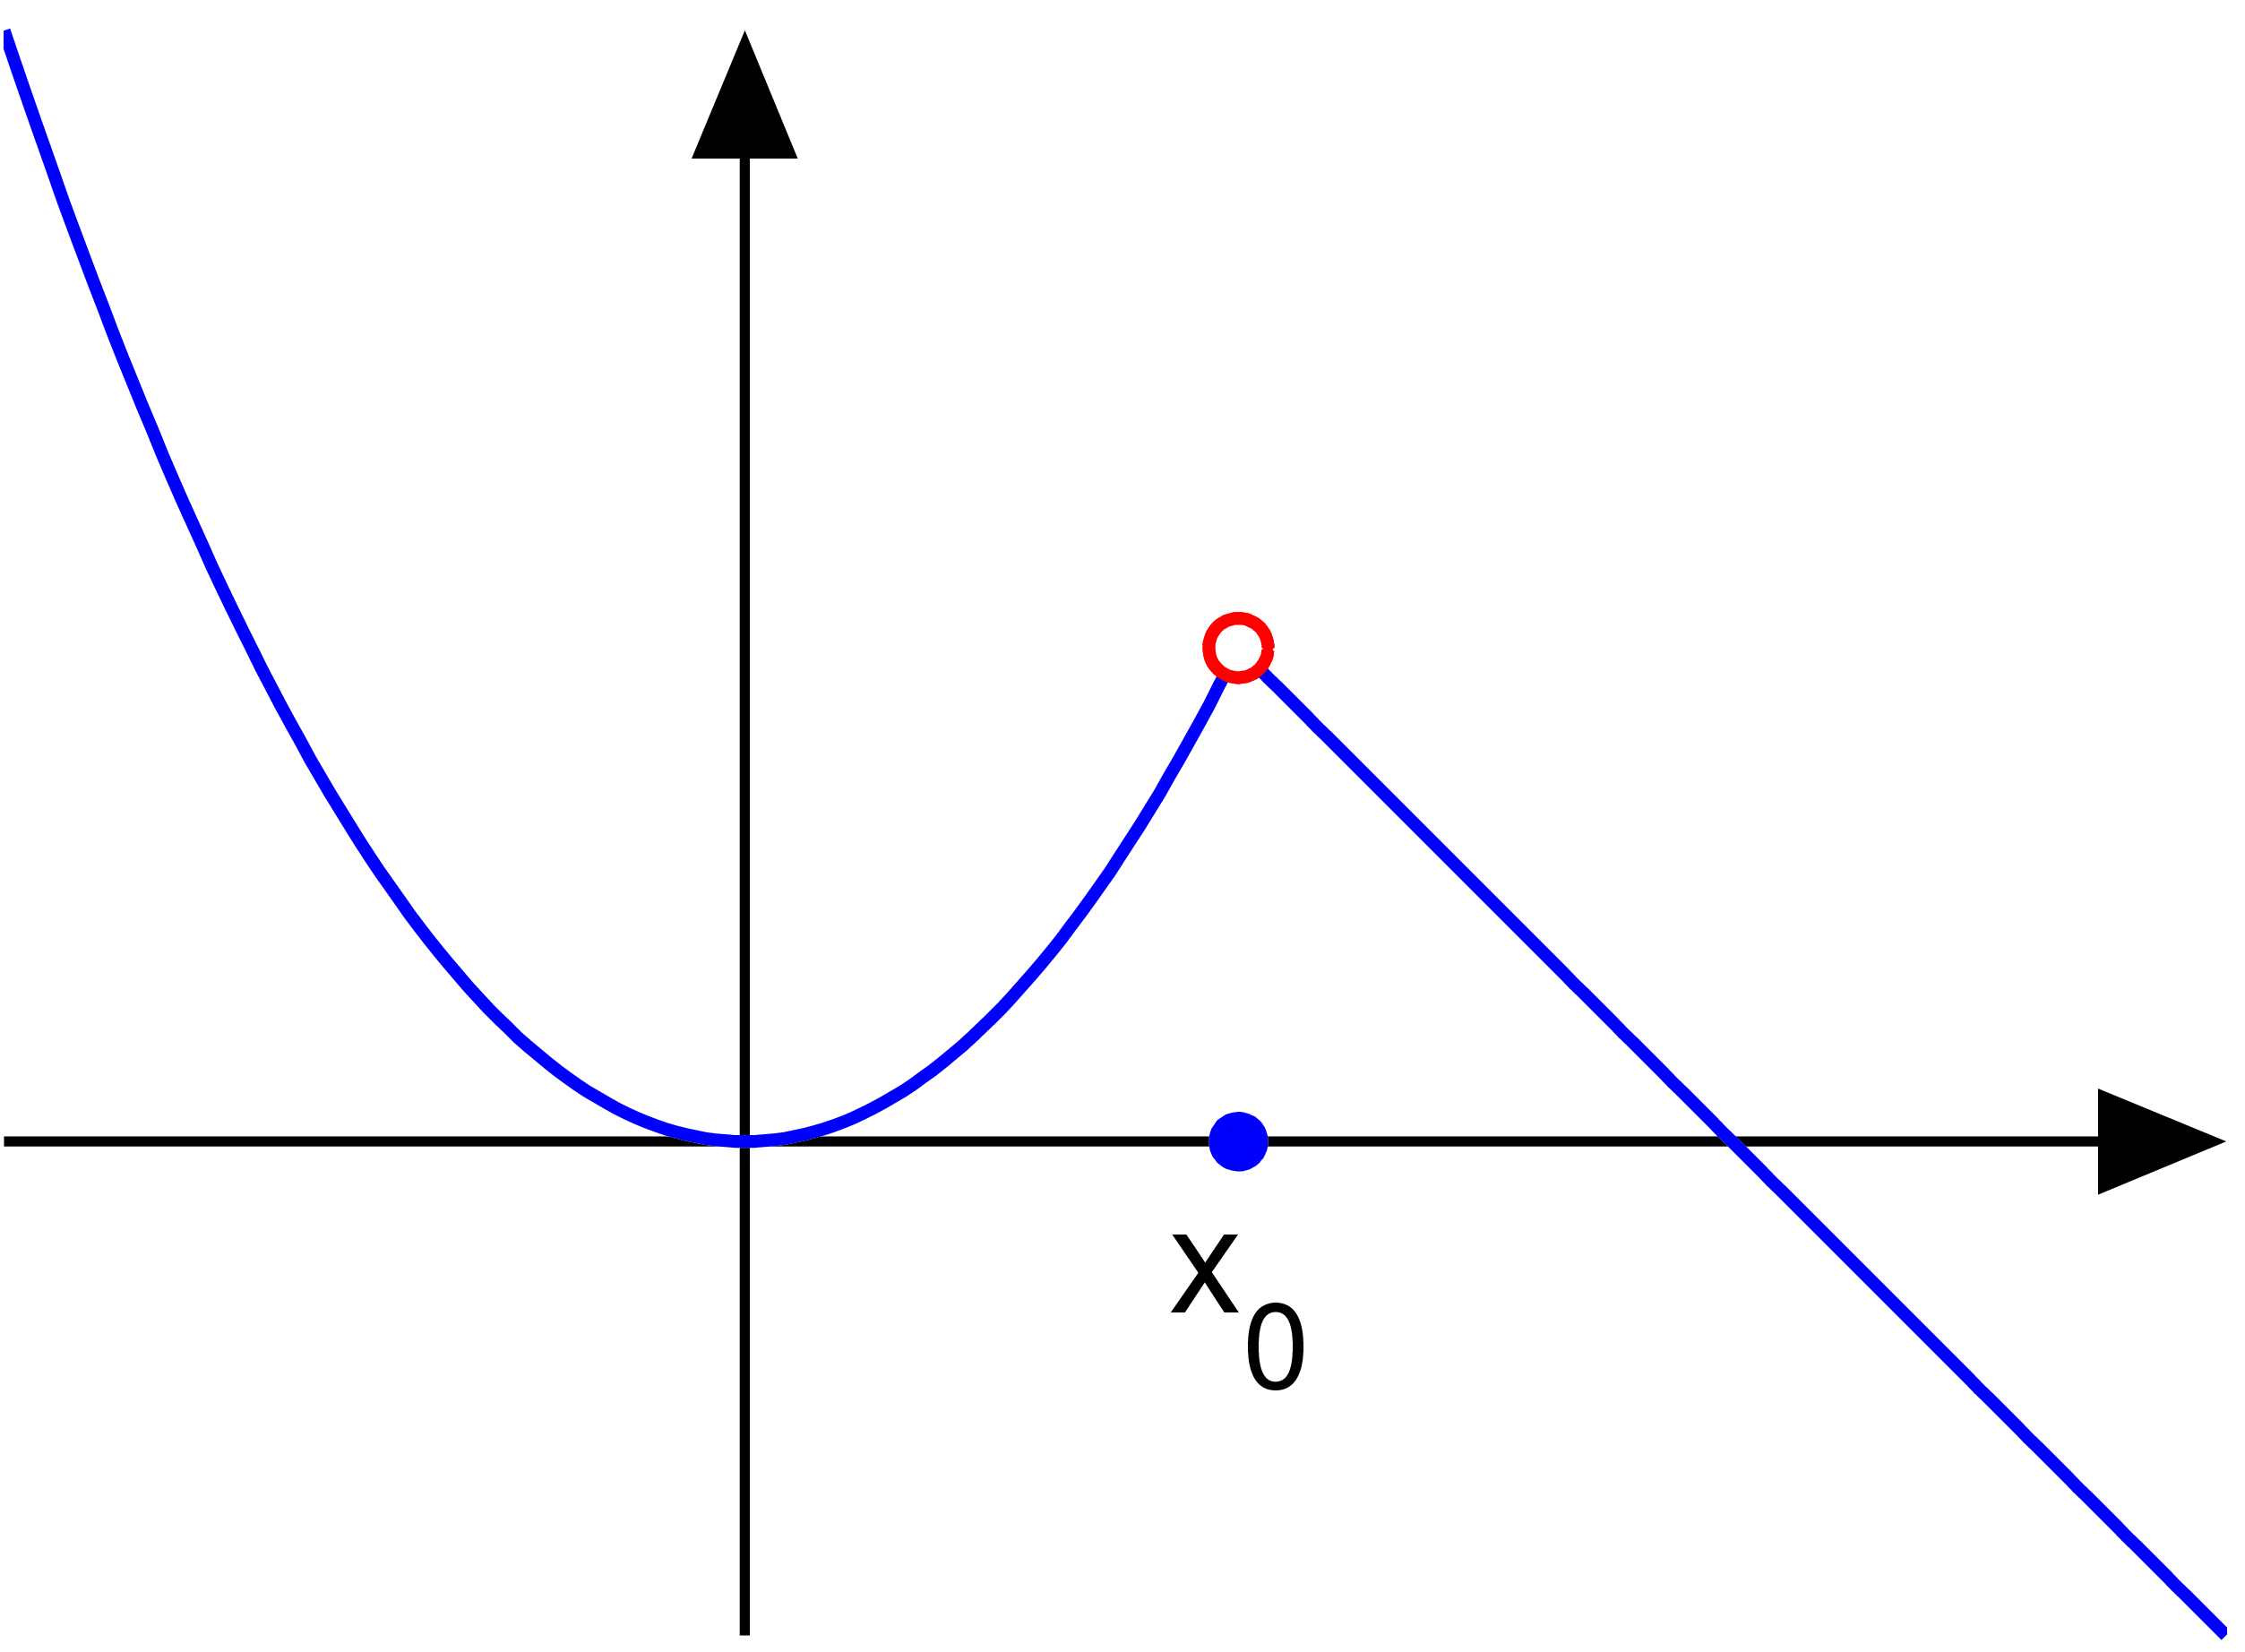
\includegraphics[width=0.3\textwidth]{\subfix{../images/Discontinuity_removable.png}}\par
  第一类不连续点,可去不连续点。
\end{figure}

\begin{figure}[h]
  \centering
  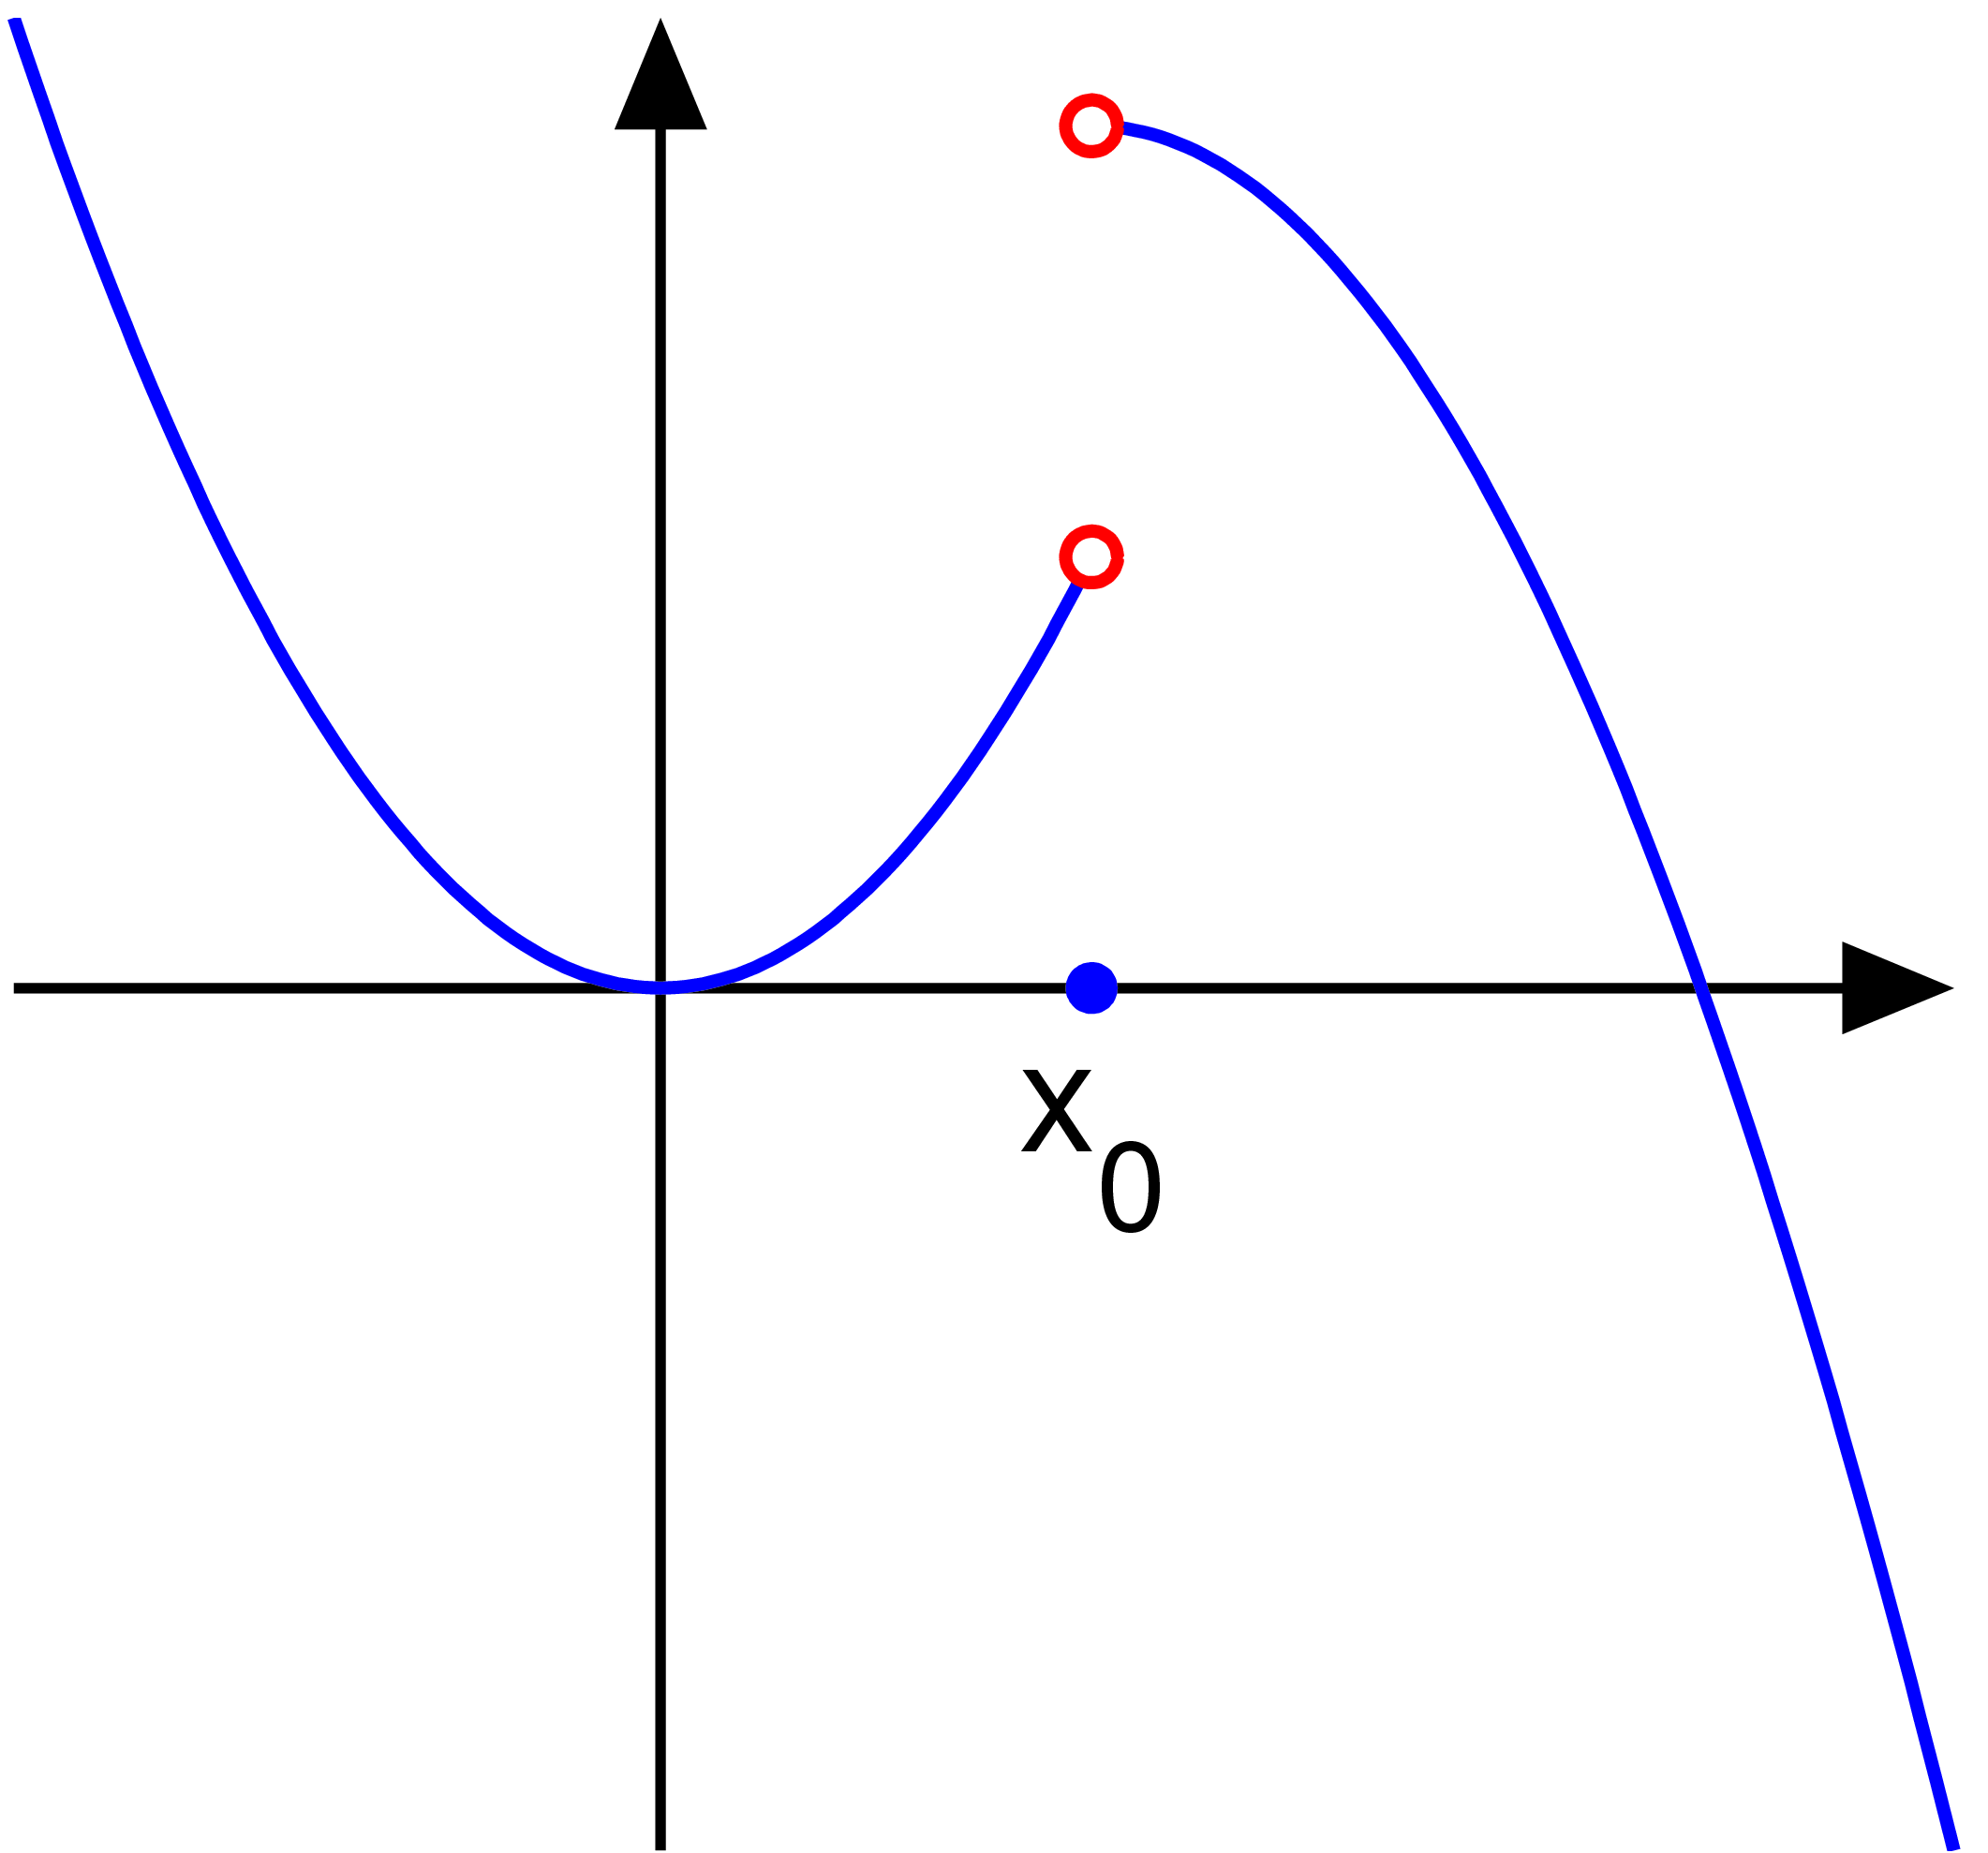
\includegraphics[width=0.3\textwidth]{\subfix{../images/Discontinuity_jump.png}}\par
  第一类不连续点,跳跃不连续点。
\end{figure}

\begin{figure}[h]
  \centering
  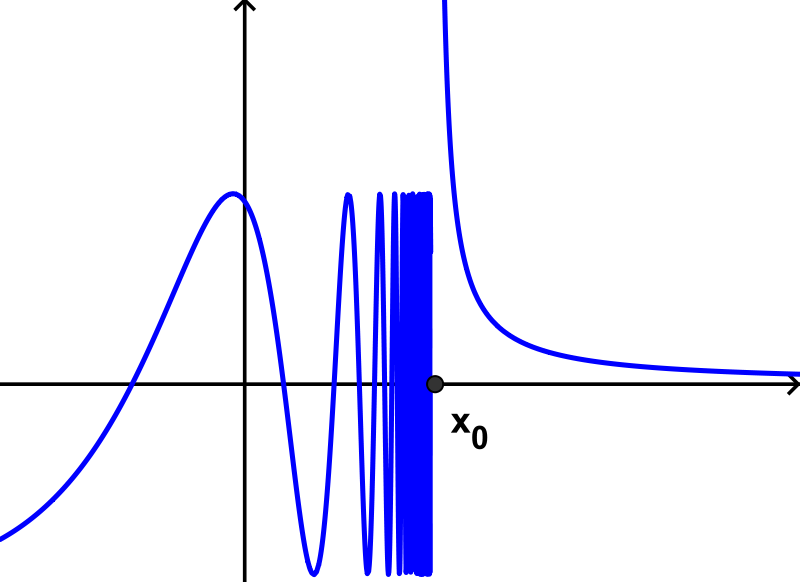
\includegraphics[width=0.3\textwidth]{\subfix{../images/Discontinuity_essential.png}}\par
  第二类不连续点(本性不连续点),可进一步分为无穷不连续点和震荡不连续点。
\end{figure}

\begin{examples}
  \begin{enumerate}[label=(\alph*)]
    \item Define
          \[
            f(x) =
            \begin{cases}
              1 & (x \ \text{rational}),   \\
              0 & (x \ \text{irrational}).
            \end{cases}
          \]
          Then $f$ has a discontinuity of the second kind at every point $x$, since neither $f(x+)$ nor $f(x-)$ exists.
    \item Define
          \[
            f(x) =
            \begin{cases}
              x & (x \ \text{rational}),   \\
              0 & (x \ \text{irrational}).
            \end{cases}
          \]
          Then $f$ is continuous at $x = 0$ and has a discontinuity of the second kind at every other point.
    \item Define
          \[
            f(x) =
            \begin{cases}
              x + 2  & (-3 < x -2),    \\
              -x - 2 & (-2 \le x < 0), \\
              x + 2  & (0 \le x < 1).
            \end{cases}
          \]
          Then $f$ has a simple discontinuity at $x = 0$ and is continuous at every other point of $(-3, 1)$.
    \item Define
          \[
            f(x) =
            \begin{cases}
              \sin\frac{1}{x} & (x \ne 0), \\
              0               & (x = 0).
            \end{cases}
          \]
          Since neither $f(0+)$ nor $f(0-)$ exists, $f$ has a discontinuity of the second kind at $x = 0$. We have not yet shown
          that $\sin x$ is a continuous function. If we assume this result for the moment, Theorem 4.7 implies that $f$ is
          continuous at every point $x \ne 0$.
  \end{enumerate}
\end{examples}

\end{document}

